\section{Hybrid positioning and Kalman filter}

%TODO: Quite = more accucate than absolute and relative?
The absolute positioning method is quite accurate but still it suffers from noise. On the other hand relative position has a lot of uncertainty, because of the physical interference. By combing these two positioning methods we can get more a precise location based on sensor measurements from absolute and predictions from the relative positions. This combination is called hybrid positioning. One of the methods using this kind of technique is the Kalman filter, which this section describes.

The Kalman filter was made by Rudolf E. Kalman in 1960. It was developed for the Apollo 11 mission\footnote{\cite{Grewal2010}} to the moon to track the location of the space shuttle. This method is still used, because it dos not require a lot of processing power or memory space. This is because the method does not need to save any data apart from the model of movement and and previous position.

The process of the Kalman filter is as follows:

%TODO: We need to describe what the model is - how is it made?
\begin{enumerate}
	\item 1. Predict the position from previous position and movement of the model.
	\item 2. Correct the position from the measured data.
	\item 3. Repeat step 1 and 2.
\end{enumerate}

Figure \ref{fig:KalmanfilterRotation} shows this visually.

\begin{figure}[H]
	\centering
	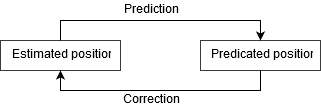
\includegraphics[width=0.4\linewidth]{positioning/positioning/KalmanFilterProcess}
	\caption{The workings of the Kalman filter.}
	\label{fig:KalmanfilterRotation}
\end{figure}

In figure \ref{fig:Kalmanfilter} two cases are shown of how the filter works. First one is at time(T-1) and time(T). In this case the filter gets closer to the measured Gaussian distribution, because it is more reliable. The hybrid position probability is higher than absolute and relative positioning. This is because the distribution of these two are multiplied together. The second case is at time (T) and (T+1). In this case the measurements have a lot more noise to them, so the estimation distribution is moving further from the measurement distribution, because of the lower probability. 

\begin{figure}[H]
	\centering
	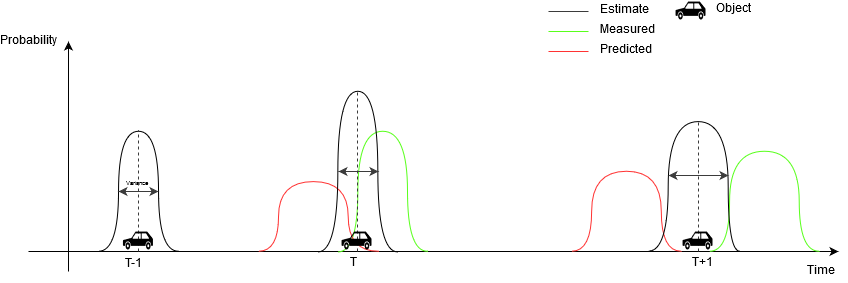
\includegraphics[width=0.7\linewidth]{positioning/positioning/DiagramKalman}
	\caption{Kalman filter example.}
	\label{fig:Kalmanfilter}
\end{figure}